\documentclass[12pt]{article}
\title{Comparison of Convolutional Neural Networks for Remote Sensing}
\date{2018-05-09}
\author{James Hurt}
\usepackage[margin=1.0in]{geometry}
\usepackage{graphicx}
\usepackage{subcaption}
\usepackage{cleveref}
\usepackage{indentfirst}
\usepackage{amsmath}
\usepackage{siunitx} % Required for alignment

\begin{document}
	\pagenumbering{arabic}
	
	%%%%%%%%%%%%%%%%
	% Title 
	%%%%%%%%%%%%%%%%
	\begin{flushright}
		James Hurt\break
		CS 8780\break
		9 May 2018
	\end{flushright}
	\begin{center}
		\huge{Comparison of Convolutional Neural Networks for Remote Sensing}
	\end{center}
	
	%%%%%%%%%%%%%%%%%%%%%%%
	% Technical Description
	%%%%%%%%%%%%%%%%%%%%%%%

	\begin{figure}[b!]
			\centering
			\begin{subfigure}[b]{0.3\linewidth}
				\centering
				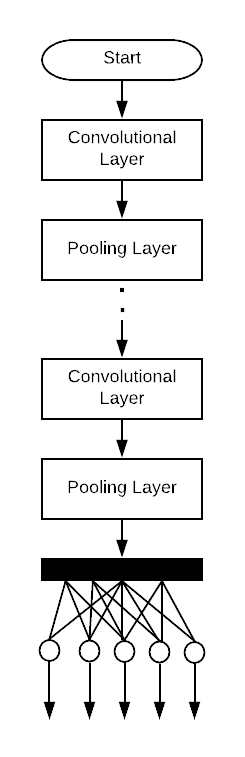
\includegraphics[scale=0.38]{img/custom_arc.png}
				\caption{Custom Shallow CNN}
				\label{fig:shallow_cnn}
			\end{subfigure}
			\begin{subfigure}[b]{0.3\linewidth}
				\centering
				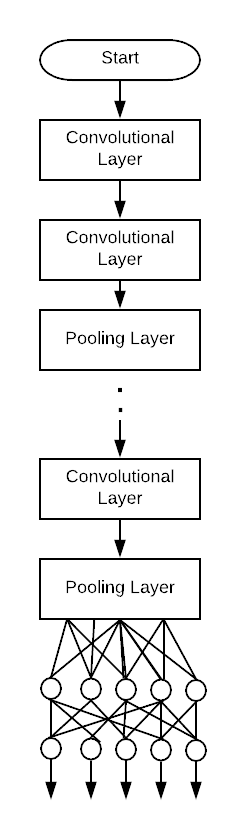
\includegraphics[scale=0.34]{img/vgg.png}
				\caption{VGG19}
			    \label{fig:deep_cnn}
			\end{subfigure}
			\begin{subfigure}[b]{0.3\linewidth}
				\centering
				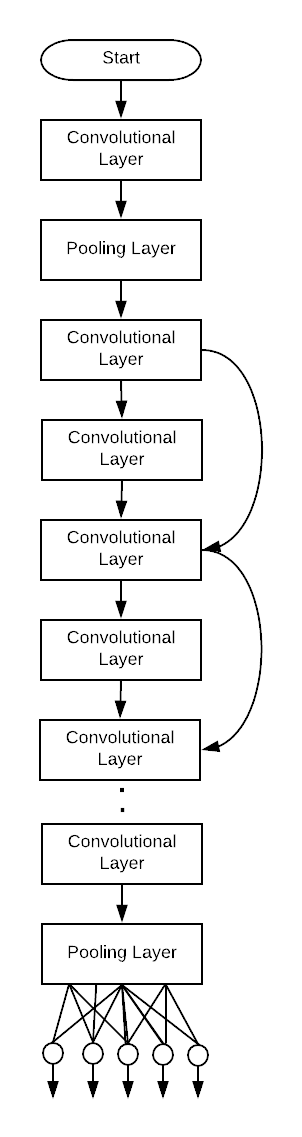
\includegraphics[scale=0.25]{img/res50.png}
				\caption{ResNet-50}
				\label{fig:deep_rnn}
			\end{subfigure}
			\caption{Architectures of the Compared CNN}
			\label{fig:architecture}
		\end{figure}

	\section{Technical Description}
	
Remote Sensing is a lucrative application for computational intelligence, with much of the recent research being in Convolutional Neural Networks. Within this discussion of neural networks for remote sensing, Deep Convolutional Neural Networks (DCNN) are the most popular. The popularity of convolutional neural networks can be attributed to the ability of a convolutional network to learn the features of the image, thus eliminating one of the greatest challenges in all of machine learning: feature selection and extraction. While CNN have proven very useful, one of the issues with DCNN is the high training time, even with GPU acceleration. In this project, I attempt to compare a shallow convolutional network with one of the first deep convolutional networks. I then take my comparison one step farther, by looking at the relative cost and benefit of residual neural networks. 
		
I chose to make my comparison of CNN for the application of Remote Sensing because I am very interested in Remote Sensing. I think the ability to detect object from satellite imagery has many applications in every day life and can better the lives of common people as well as aid industry in understanding what is around their facilities. 
		
		\subsection{Shallow Convolutional Neural Network}
		
The shallow convolutional neural network used in this project combines many techniques of fully connected networks previously used for pattern recognition. The architecture of the network can be see in \Cref{fig:shallow_cnn}.
		
The architecture of the network has a total of 12 layers. The first 10 layers are alternating 2D Convolutional layers with a 3x3 kernel size and 2D Max Pooling layers with a 2x2 Pooling Window. After these 10 layers, feature extraction is finished. I then added a flattening layer because the fully connected layer required a 1D vector as input. I then add the fully connected layer with a softmax activation function for classificaion.
		
		
		\subsection{Deep Convolutional Neural Network}
		
The Deep Convolutional Neural Network used for comparison in this project is VGG19 \cite{vgg}. The VGG19 network, as the name suggests, has 19 total layers. This count, however, does not include the pooling layers. The basic architecture can been seen in \Cref{fig:deep_cnn}. 

VGG19 has 16 convolutional layers and 4 pooling layers. The interesting quality about VGG19 is that the final pooling layer does not connect directly to the softmax output layer. Instead, the final pooling layer's output if flattened and used an input for a 3-layer multilayer perceptron (MLP) \cite{ci_book} The final layer of this MLP is a softmax layer for classification. 

		\subsection{Deep Residual Convolutional Neural Network}

The final neural network used for comparison in this project is a Deep Residual Convolutional Neural Network (DRNN). I chose to use ResNet-50 \cite{resnet50}, a standard DRNN for comparison developed by Microsoft Research. The architecture of this network can be seen in \Cref{fig:deep_rnn}.

ResNet-50 begins with a single convolutional layer, followed by a single pooling layer. After the initial pooling layer, there are 49 convolutional layers that are \textit{residual}, meaning that there is a connection from layer \textit{N} to both layer \textit{N+1} as well as layer \textit{N+2}. This connection exists so that the error from the two connections to the \textit{N+2} layer can be summed when performing backpropagation, thus slowing the disappearance of the gradient. Deep RNN's have gained so much popularity due to this feature of relieving the disappearing gradient. This issue occurs when training deep networks because as weight vector approaches the minimum, the gradient is so small that there is not very much update to the weights, so the minimum may never be reached. By summing the error from several previous layers, the gradient disappear slower, allowing a more flexible and better performing network. 
	
	\section{Algorithm Design}
	
	\begin{figure}[t!]
		\centering
		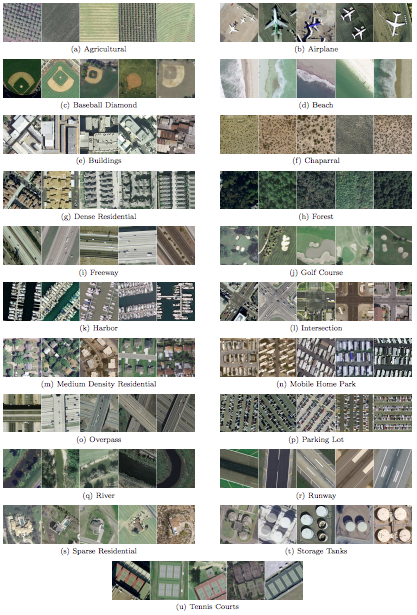
\includegraphics[width=0.5\linewidth]{img/ucm.png}
		\caption{UCMerced Dataset with 21 classes}
		\label{fig:ucm}
	\end{figure}
	
	\subsection{Dataset Selection}
The algorithm I designed for comparing these various CNN involved 2 datasets: a 3 class dataset and the benchmark UC Merced Dataset \cite{ucm}. The 3 class problem is a subset of the UCMerced dataset. I chose 3 classes from the UCMerced dataset: agricultural, airplane, and baseball diamond. While the test dataset is small, the UCMerced dataset, seen in \Cref{fig:ucm} is not. It has 21 classes, each with 100 images each. This dataset is not the largest available as far as benchmark Remote Sensing is concerned, but I felt it was a good representative for my comparison, because I didn't want too challenging a dataset. 

I chose to use 2 datasets because I felt that using only one would not give me enough of a picture to draw conclusions. Perhaps, if I had chosen just one dataset, the dataset I picked was particularly suited to one of these methods, but if I chose 2, then I would have enough to draw somewhat of a conclusion. Certainly, only 2 datasets is not enough for a generalization, but it does allow me to eliminate the possibility of choosing a biased dataset.

I also chose to have a small and large dataset, because there are many instances of binary classification needed in everyday life, so looking at a 3 class problem as well as a large, 21 class problem, would allow me to see if one method was better for large but not small or vice versa. If I found that the shallow could better handle the 3 class problem or maybe if the shallow CNN was within 1\% cross validation accuracy, for example, then I could say that binary classifiers could settle for a shallow CNN, thus relieving the long training times required for Deep CNN or RNN. 

	\subsection{Parameter Selection}
After choosing the datasets to use, I had to decide on the parameters for the algorithms. The choices I had to make specifically were the loss function and the optimizer. I needed to choose one of each that would be used in all 3 algorithms. I had to use the same one to ensure a fair comparison. 

The loss function I decided to use was \textbf{categorical crossentropy} \cite{cross_entropy}: 
		
\[
		H(q,p) =  \int q(x) log(q(x) / p(x)) \mathrm{d}x
\]

Crossentropy, as discussed in the first Computational Intelligence class, is a useful loss function because it harshly punishes output that is very far from the correct value. It is more punishing than standard error and can help a network converge in less epochs. 

For the optimizer, I started with knowledge of gradient descent from the previous Computational Intelligence class, and decided to choose a similar optimizer for my CNN, \textbf{Stochastic Gradient Descent (SGD)} \cite{sgd}:

\[
	w(t+1) = w(t) - \eta \frac{\partial}{\partial w} \ell(f(x_t), y_t)
\]

The function of SGD is very similar to gradient descent in that we are attempting to move the opposite direction of the error function in search of a set of parameters such that there exists a global minimum for error.

	\subsection{Comparison Algorithm}
	
To compare the three algorithms, I designed two separate Python classes to utilize the Tensorflow GPU and Keras libraries for Deep Learning. The first class was for the shallow CNN. I manually defined the 12 layers for the model, as well as built general utility functions to take in a directory of images and generate the 5 folds and to take in a list of filenames and generate an array of 3D matrices that were the normalized, numerical representations of the images required by Keras for training the networks. After defining these functions, I build logic to run a cross validation experiment. on the given images and storing results in a variable for later use.

Once I had the shallow network build and working, I built another class for the 2 deep networks: VGG19 and ResNet-50. This class utilized many of the functions I wrote for the shallow network. The main difference was the model. For the shallow, I had to build the model from scratch. For these networks, I was able to import the convolutional and pooling layers from Keras. I only had to build the final layer for classification with a softmax activation function and attach it to the end of the final convolutional layer. I only needed 1 class for both networks because I could pass a boolean to the class to tell it whether to import ResNet-50 or VGG19. This class also had logic to perform a cross validation experiment with 1 function call and store results for later analysis. 

After I had the ability to perform cross validation experiments with 1 function call, I built a script to bring in the two datasets, train them for 10, 20, 30, 40, and 50 epochs, and record the performance of all 3 nets on both networks for the 5 different lengths of training. One of the concerns of this project was the training time, so I feel it is important to note that all experiments were GPU accelerated with 4 Nvidia GPUs using cuDNN, a C++ CUDA library for Deep Learning on Nvidia GPUs, which was then tied into Tensorflow-GPU, which is optimized for cuDNN. 
	
	\section{Experiment Results}
	
	The experiments run were 5-fold cross validation on  both the test dataset and UCMerced for 10, 20, 30, 40, and 50 epochs on the ShallowCNN, Deep CNN (VGG19), and Deep RNN (ResNet-50)
	\subsection{Test Dataset}

	\begin{table}[h!]
		\begin{center}
			\caption{Average Cross Validation Accuracy for Test Dataset}
			\label{table:test}
			\begin{tabular}{l | S | S | S | S |  S}
				\textbf{Method} & \textbf{10 Epochs} & \textbf{20 Epochs} & \textbf{30 Epochs} & \textbf{40 Epochs} & \textbf{50 Epochs} \\
				\hline
				Shallow CNN & 91.2\% & 92.5\% & 92.2\% & 89.7\% & 92.8\% \\
				Deep CNN & 35.1\% & 33.1\% & 33.1\% & 57.7\% & 33.5\% \\
				Deep RNN & 75.5\% & 94.5\% & 92.3\% & 97.3\% & 94.9\% \\
				
			
			\end{tabular}					
		
		
		\end{center}
	
	\end{table}
	\subsection{UCMerced Dataset}
	\begin{table}[h!]
		\begin{center}
			\caption{Average Cross Validation Accuracy for UCMerced Dataset}
			\label{table:ucm}
			\begin{tabular}{l | S | S | S | S |  S}
				\textbf{Method} & \textbf{10 Epochs} & \textbf{20 Epochs} & \textbf{30 Epochs} & \textbf{40 Epochs} & \textbf{50 Epochs} \\
				\hline
				Shallow CNN & 38.9\% & 38.6\% & 35.3\% & 26.6\% & 33.2\% \\
				Deep CNN & 17.9\% & 15.1\% & 18.6\% & 4.9\% & 53.1\% \\
				Deep RNN & 94.8\% & 96.2\% & 96.2\% & 96.4\% & 97.8\% \\
				
			
			\end{tabular}					
		
		
		\end{center}
	
	\end{table}
	
	\section{Analysis}
	
	\begin{figure}[t!]
	\centering
		\begin{subfigure}[b]{0.4\linewidth}
			\centering
			\fbox{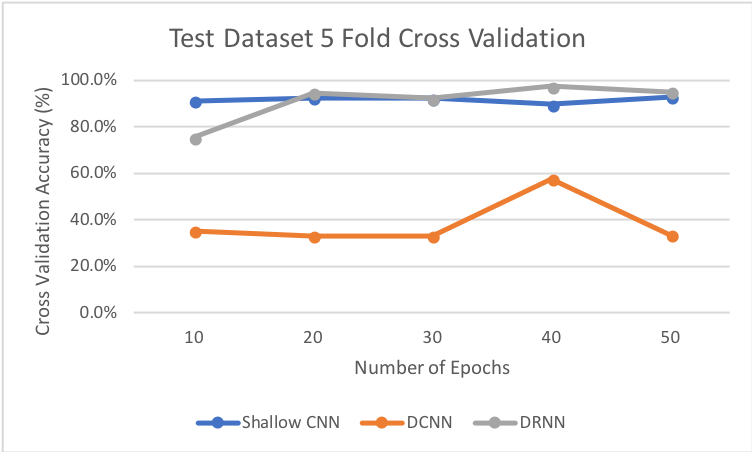
\includegraphics[width=0.93\linewidth]{img/test_dataset.png}}
			\caption{Test Dataset}	
		\end{subfigure}
		\begin{subfigure}[b]{0.4\linewidth}
			\centering
			\fbox{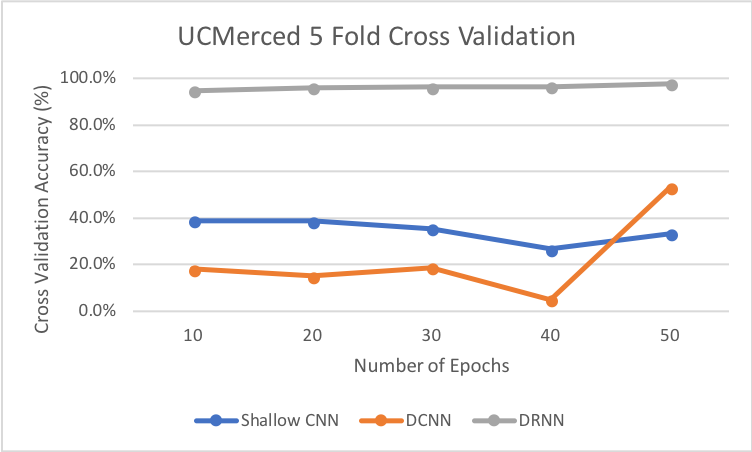
\includegraphics[width=0.9\linewidth]{img/ucmerced.png}}
			\caption{UCMerced Dataset}
			\label{fig:ucm_trend}
		\end{subfigure}
		\caption{Trends of Epochs vs Cross Validation Accuracy}
		\label{fig:result_graphs}
	\end{figure}
	
	After looking at the results in \Cref{table:test} and \Cref{table:ucm}, I was honestly shocked. I did not expect in any way to see results that were so lopsided and inconsistent. I was expecting to see some sort of trend in the models and how they perform on the two datasets, but what I found was inconsistent and, to some degree, made no sense. To try and understand the trends and inconsistency in my results, I created 2 visualizations, seen in \Cref{fig:result_graphs}. 
	
	When analyzing the graphs in \Cref{fig:result_graphs}, I was first struck by the lack of performance of the DCNN.  The best result from the DCNN was 57.7\% for 40 epochs of training on the test dataset. Every other result but 1 was below 50\%, which is honestly terrible. I do not have a lot of experience with VGG19, and I chose it because I needed a network that was not residual, but was a deep convolutional network. I suspect that my poor results for this model are indicative of a lack of preprocessing or standardization that was performed in the original VGG19 experiments. Perhaps if I do more experiments with a wider range of parameters and different methods of normalizing the data, I would find the ideal configuration for VGG19 to perform. I attempted some small experiments with different normalizations such as normalizing all pixel values between -1 and 1, and normalizing from 0 to 1, but neither of these improved performance in any way. I also think that perhaps VGG19, being only 16 convolutional layers, would benefit from more training. When looking at \Cref{fig:ucm_trend}, I saw an upward trent from 40 to 50 epochs of training. Perhaps 120 epochs, or 200 epochs, would increase my accuracy given that there was no augmentation performed. This 50 epoch training experiment on UCMerced is also the only experiment done in which VGG19 does not have the worst performance of the three compared methods. 
	
	The next major observation I had when looking over the results was the huge jump in accuracy when moving from UCMerced to the Test Dataset for the Shallow CNN. The best performance by the shallow network on the UCMerced was actually for the least amount of training, but was still only 38.9\%, which indicates a limitation of shallow networks -- more complex, or a larger number of classes, creates problems for shallow networks. Perhaps the smaller number of layers does not provide enough complexity in number of parameters to learn all the weights needed for a high cross validation score. This worsened performance of the shallow CNN also shows the need for deep networks. The Shallow CNN performed slightly better than the Deep CNN, but only for the limited training experiments. Once the number of epochs hit 50, the accuracy for the Deep CNN jumped over the Shallow CNN, which also shows the need for more epochs of training of Deep CNNs. 
	
	While the lack of performance on UCMerced shows that Shallow CNN cannot handle complex problems, the extremely high performance on the 3-class dataset shows that for binary, or limited number of class, situations, the Shallow CNN performs \textit{almost} as well as the Deep RNN. The best performance for the Test Dataset was still the Deep RNN, but even if we assume that the performance of the Shallow RNN on simpler problems is ~90\%, that may be sufficient for many applications. There are instances where the tradeoff between training time and performance may lean towards lower training time, even if that means a drop of 8-9\% of performance. The training of the Deep RNN for 50 epochs took a little over an hour with 4 GPUs, meaning that if a firm or research group did not have the infrastructure for GPU acceleration, then the time to train the Deep RNN may be overwhelming whereas training the Shallow CNN took less than 15 minutes. In those instances where resources or time are limited, Shallow CNN have their place. 
	
	In addition to understanding when Shallow CNN may prove to be the best choice, another conclusion that I made based on the results of these experiments was that when given the choice between a pure DCNN, or a Residual DCNN, always choose the Residual Network, with all things being equal. The DRNN consistently performed better than either of the other models, and more importantly, it was by far the most consistent and dependable model that I examined. The only experiment run for which the DRNN did not have > 90\% accuracy was with 10 epochs of training on the Test Dataset, which is remarkable. For all experiments with number of epochs greater than or equal to 20, accuracy for the DRNN on both large and small problems, was at least 92.3\%. The residual network was well worth the extra training for my problem because I was able to GPU accelerate, so the extra time to train was worth it for the boost from 33.2\% to 97.8\% for 50 epochs on UCMerced. 
	
	In conclusion, when comparing 5-class cross validation classification accuracy for Shallow CNN, Deep CNN, and Deep RNN in a 3-class problem and 21-class problem, the Shallow CNN is best used for a small number of classes when resources or time are limited and perhaps when time to solution is worth a drop of ~10\% in performance. The Deep CNN did not perform well at all with the chosen parameters, but perhaps more experimentation with loss, optimizer, normalization, or length of training would lead to a jump in accuracy across 5-fold cross validation. The jump in training time for the Deep CNN did not prove to be wise, as in only 1 of the 10 experiments was the Deep CNN not the worst performing model. Finally, in cases where high accuracy is the most important and/or when there are sufficient resources for GPU acceleration, the Deep RNN is the safest and most reliable choice for Remote Sensing. While the hours of extra training only yielded ~5\% improvement of accuracy for the 3-class dataset, the Deep RNN is still the safest and most consistent choice for CNN within applications of Remote Sensing. 
	
	\section{Code}
	
	This project was developed using Python3 and has a high number of dependencies for running, including the Deep Learning libraries TensorFlow and Keras. Please note that training the Deep CNN or Deep RNN without GPU Acceleration will most likely take several hours. The code for this project can be seen in the \textbf{Code} folder. Please see the \textit{README.md} file within that folder for instructions on how to run the project.  
	
	
%%%%%%%%%%%%%%%%
%		 REFERENCES
%%%%%%%%%%%%%%%%%
	\newpage
	\bibliography{bibliography} 
	\bibliographystyle{ieeetr}




\end{document}